% These appendices collect supplementary figures and tables referenced from
% the main text but not reproduced there, grouped by the chapter they support.

\chapter{Data}
\label{app:data-dictionary}

The downloaded raw-data directory contains 186 annual CSV files from 26 logical dataset families.
The tables below document the EC variables and project-derived features used by the modelling
pipeline. The annual files are not perfectly schema-uniform: the 2017 greenhouse-gas
file has a malformed header containing appended unit fields, subsequent greenhouse-gas files place
units in a separate first data row, and the environmental-measurement schema decreases from 718 to
694 columns from 2022 as phosphorus streams for several catchments disappear. Annual query windows
also overlap at some boundary timestamps. Compilation therefore removes duplicated timestamps and
normalises the time index before hourly aggregation. The greenhouse-gas record ends on 1 January
2024, so its substantive observations cover 2017--2023. Later records are available for environmental,
livestock and management sources, but not for EC fluxes.

{
\scriptsize
\setlength{\tabcolsep}{2pt}
\renewcommand{\arraystretch}{1.14}
\setlength\LTleft{0pt}
\setlength\LTright{0pt}
\begin{longtable}{p{2.7cm}p{4.5cm}p{2.5cm}p{4.8cm}}
\caption{Complete base-variable dictionary for the raw eddy-covariance, biomet and turbulence files. Each listed base variable is repeated for Towers 2, 4 and 9. Definitions, units and native resolution follow the NWFP EC greenhouse-gas guide \cite{olde2023ec}; treatment and analytical role describe processing in this project. Tower identifiers and repeated suffixes are omitted for readability.}
\label{tab:ch3_ec_dictionary}\\
\toprule
Variable & Meaning & Unit and resolution & Treatment and analytical role \\
\midrule
\endfirsthead
\multicolumn{4}{l}{\tablename\ \thetable\ -- continued}\\
\toprule
Variable & Meaning & Unit and resolution & Treatment and analytical role \\
\midrule
\endhead
\midrule
\multicolumn{4}{r}{Continued on next page}\\
\endfoot
\bottomrule
\endlastfoot
\texttt{CO2} & Carbon-dioxide mole fraction measured by the gas analyser & mmol CO\textsubscript{2} mol$^{-1}$; 30 min & Available raw concentration; not retained as a direct model feature \\
\texttt{H2O} & Water-vapour mole fraction measured by the gas analyser & mmol H\textsubscript{2}O mol$^{-1}$; 30 min & Available raw concentration; not retained directly \\
\texttt{CH4} & Methane mole fraction measured by the gas analyser & nmol CH\textsubscript{4} mol$^{-1}$; 30 min & Distinct from ecosystem-scale methane flux; not retained directly \\
\texttt{TAU} and \texttt{TAU\_SSITC\_TEST} & Momentum flux and its steady-state/integral-turbulence quality class & kg m$^{-1}$ s$^{-2}$ and categorical; 30 min & Available turbulence output; not retained directly \\
\texttt{H} and \texttt{H\_SSITC\_TEST} & Sensible-heat flux and its quality class & W m$^{-2}$ and categorical; 30 min & Available energy-balance output; not retained directly \\
\texttt{LE} and \texttt{LE\_SSITC\_TEST} & Latent-heat flux and its quality class & W m$^{-2}$ and categorical; 30 min & Available energy-balance output; not retained directly \\
\texttt{FC} (FCO\textsubscript{2}) & Net ecosystem carbon-dioxide exchange & $\mu$mol CO\textsubscript{2} m$^{-2}$ s$^{-1}$; 30 min & Carbon-cycle predictor and partitioning input; values outside $[-100,100]$ are rejected \\
\texttt{FC\_SSITC\_TEST} & SSITC quality class for each carbon-dioxide-flux estimate & Categorical: 0 high, 1 medium, 2 low quality; 30 min & Classes 0 and 1 are retained before FCO\textsubscript{2} reconstruction \\
\texttt{FCH4} (FCH\textsubscript{4}) & Methane flux measured by eddy covariance & nmol CH\textsubscript{4} m$^{-2}$ s$^{-1}$; 30 min & Prediction target; classes 0 and 1 are retained and fluxes outside $[-500,3000]$ are treated as missing \\
\texttt{FCH4\_SSITC\_TEST} & SSITC quality class for each methane-flux estimate & Categorical: 0 high, 1 medium, 2 low quality; 30 min & Provider quality field used to screen the target \\
\texttt{WD} & Horizontal wind direction & degrees; 30 min & Converted to sine and cosine components when used in forecasting \\
\texttt{WS}/\texttt{WS\_MAX} & Mean and maximum horizontal wind speed & m s$^{-1}$; 30 min & Mean wind speed is retained; the maximum is available but not retained \\
\texttt{U/V/W\_SIGMA} & Standard deviations of the three wind components & m s$^{-1}$; 30 min & Available turbulence diagnostics; not retained directly \\
\texttt{USTAR} & Friction velocity representing atmospheric turbulence & m s$^{-1}$; 30 min & Predictor and diagnostic; values outside $[0,3]$ are removed, while the derived low-turbulence flag is not applied to FCH\textsubscript{4} \\
\texttt{MO\_LENGTH}/\texttt{ZL} & Monin--Obukhov length and dimensionless stability ratio $z/L$ & m and dimensionless; 30 min & Available atmospheric-stability diagnostics; not retained directly \\
\texttt{FETCH\_MAX}, \texttt{FETCH\_70/80/90} & Maximum fetch and distances containing 70, 80 and 90\% of the modelled footprint contribution & m; 30 min & Available footprint diagnostics; not retained as model features \\
\texttt{PA} & Atmospheric pressure & kPa; 30 min & Available meteorological variable; not retained directly \\
\texttt{RH\_0}/\texttt{RH\_1} & Relative humidity measured by the EC and biomet systems & \%; 30 min & Available but excluded from retained feature sets in favour of VPD \\
\texttt{TA\_0} (TA) & Air temperature & $^{\circ}$C; 30 min & Meteorological predictor and carbon-partitioning input; an external series is available \\
\texttt{VPD} & Vapour-pressure deficit, representing atmospheric moisture demand & hPa; 30 min & Retained predictor; a $[0,15]$\,hPa plausibility bound
  is applied before gap-filling to remove implausible
  outlier readings \\
\texttt{T\_SONIC} and sigma & Sonic temperature and its \texttt{T\_SONIC\_SIGMA} standard-deviation field & $^{\circ}$C; 30 min & Available sonic-anemometer outputs; not retained directly \\
\texttt{LWIN}/\texttt{LWOUT} & Incoming and outgoing long-wave radiation & W m$^{-2}$; 30 min & Available radiation components; not retained directly \\
\texttt{PPFD} & Incoming photosynthetic photon-flux density & $\mu$mol photons m$^{-2}$ s$^{-1}$; 30 min & Radiation and plant-activity predictor \\
\texttt{RN} & Net radiation at the land surface & W m$^{-2}$; 30 min & Surface-energy predictor \\
\texttt{SHF\_1/2/3} & Soil heat flux recorded by three plates & W m$^{-2}$; 30 min & Sensor 1 is retained in the base feature set; all three are averaged in selected forecasting configurations \\
\texttt{SWC\_1/2/3} & Volumetric soil-water content from three EC-biomet sensors & m$^{3}$ m$^{-3}$; 30 min & Available EC soil measurements; the adopted configuration instead uses catchment SMS observations \\
\texttt{SWIN}/\texttt{SWOUT} & Incoming and outgoing short-wave radiation & W m$^{-2}$; 30 min & Incoming radiation is retained; outgoing radiation is not retained directly \\
\texttt{TA\_1} & Secondary biomet air-temperature measurement & K; 30 min & Available raw measurement; not retained directly \\
\texttt{TS\_1/2/3} & Soil temperature from three EC-biomet sensors & K; 30 min & Sensor 1 at Tower 9 supplies the cross-tower proxy only in the EC-only configuration; adopted catchment SMS temperatures are in $^{\circ}$C \\
\end{longtable}
}

% Table disabled: detailed non-EC raw-input dictionary.
\iffalse
{
\scriptsize
\setlength{\tabcolsep}{2pt}
\renewcommand{\arraystretch}{1.14}
\setlength\LTleft{0pt}
\setlength\LTright{0pt}
\begin{longtable}{p{3.2cm}p{4.2cm}p{2.5cm}p{4.6cm}}
\caption{Dictionary of raw environmental, catchment, site-wide meteorological, livestock-count and field-event records. SMS definitions follow \cite{hawkins2023sms}, site-wide meteorology follows \cite{hawkins2023met}, hydrology and water quality follow the Data Guide \cite{hawkins2025}, and event definitions follow \cite{hawkins2023fieldevents}. Livestock-count descriptions are based on the downloaded files because a dedicated local livestock guide is unavailable.}
\label{tab:ch3_catchment_dictionary}\\
\toprule
Variable or record & Meaning & Unit and resolution & Treatment and analytical role \\
\midrule
\endfirsthead
\multicolumn{4}{l}{\tablename\ \thetable\ -- continued}\\
\toprule
Variable or record & Meaning & Unit and resolution & Treatment and analytical role \\
\midrule
\endhead
\midrule
\multicolumn{4}{r}{Continued on next page}\\
\endfoot
\bottomrule
\endlastfoot
Flume flow and pump status & Discharge derived from the instrumented catchment flume and the associated pump on/off state & L s$^{-1}$ and binary; 15 min & Flow is aggregated to hourly or daily means for extended experiments; pump status is not retained \\
Water temperature & Temperature measured in the flume and in the water-quality flow cell & $^{\circ}$C; 15 min & Available hydrological diagnostics; not retained in the base analytical feature set \\
Inorganic nitrogen chemistry & Nitrite plus nitrate, ammonia and ammonium concentrations & mg L$^{-1}$; 15 min & Available water-quality measurements; not retained in the base analytical feature set \\
Phosphorus chemistry & Total and orthophosphorus concentrations & mg L$^{-1}$; 15 min & Not retained; streams for Catchments 2, 3, 5 and 8 disappear from the downloaded schema from 2022 \\
Conductivity and dissolved oxygen & Electrical conductivity and percentage oxygen saturation & $\mu$S cm$^{-1}$ and \%; 15 min & Available water-quality measurements; not retained \\
pH, turbidity and fluorescent DOM & Acidity, optical turbidity and fluorescent dissolved organic matter & dimensionless, FNU and $\mu$g L$^{-1}$ QSU; 15 min & Available water-quality measurements; not retained \\
Catchment precipitation & Tipping-bucket precipitation recorded at the soil-moisture station; the gauge resolves 0.2 mm per tip & mm; 15 min & Aggregated hourly or to daily totals and matched only to the corresponding tower \\
Soil moisture at 10 cm & Volumetric soil-water content measured by capacitance at 10 cm & \%; 15 min & Aggregated to hourly means and used as a soil-condition predictor \\
Soil temperature at 15 cm & Soil temperature measured by the catchment soil-moisture station at 15 cm depth & $^{\circ}$C; 15 min & Aggregated to hourly means and used as a soil-condition predictor \\
Site precipitation & Precipitation measured by the dedicated site-wide meteorological station & mm; 15 min & External meteorological input; reported using a tipping bucket before 2015 and a weighing gauge thereafter \\
Site air temperature and RH & Air temperature and relative humidity measured by the dedicated meteorological station & $^{\circ}$C and \% RH; 15 min & Air temperature is adopted as an external input; relative humidity is available but not retained \\
Site wind speed and direction & Wind measured at 3 m height & km h$^{-1}$ and degrees; 15 min & Speed is divided by 3.6 before use; direction is available but the retained circular encoding uses EC wind \\
Site solar radiation & Incoming solar radiation measured by pyranometer & W m$^{-2}$; 15 min & Adopted external short-wave-radiation input \\
Provider \texttt{Quality} & Categorical validity assessment accompanying every environmental measurement series & Categorical; 15 min & Values include Acceptable, Not set, Outlier and Suspicious, with additional sensor-specific categories; these strings are currently discarded during numeric consolidation rather than applied as filters \\
Provider \texttt{Quality Last Modified} & Timestamp recording the most recent change to the corresponding quality assessment & Timestamp; 15 min & Retained in the raw files but discarded during numeric consolidation \\
Cattle, breeding-sheep and lamb counts & Numbers of each livestock class recorded at each catchment, shed and other listed location & head count; daily & The three \texttt{Animal\_location\_counts} families are expanded to the hourly index; Catchments 2, post-2013 Catchment 4 and 9 are selected \\
Event date and time fields & \texttt{Event\_Date}, entry/exit times and calculated time in field & Date, time and duration; event based & Establish the timing of a management record; date is used to construct recency features \\
Field and machinery fields & Field identifier, tractor, operator, and start, end and total tractor hours & Identifiers and hours; event based & Field identifiers are mapped to catchments; machinery metadata are not retained \\
Operation and application fields & \texttt{Field\_Operation} and \texttt{Application} descriptions & Categorical; event based & Raw records span fertiliser, pesticide, drainage, mowing, harvest, cultivation and other operations \\
Application quantity fields & Total application, units, application information, rate per hectare and batch number & Mixed units; event based & Used only where the operation and unit permit a defensible management feature \\
Product fields & Product name and manufacturer & Text; event based & Used by later corrected fertiliser processing to distinguish products and infer true nitrogen content \\
Derived management channels & Cutting, manure, fertiliser-classified, liming and cultivation histories classified from the raw event fields & Project-defined event categories & Cutting and manure recencies are retained in the pruned gap-filling set; the generic fertiliser classifier is not necessarily equivalent to confirmed nitrogen application \\
\end{longtable}
}
\fi

{
\scriptsize
\setlength{\tabcolsep}{2pt}
\renewcommand{\arraystretch}{1.14}
\setlength\LTleft{0pt}
\setlength\LTright{0pt}
\begin{longtable}{p{2.8cm}p{4.4cm}p{2.7cm}p{4.6cm}}
\caption{Dictionary of principal project-derived variables. These are not original NWFP portal columns: their definitions follow the repository's preprocessing and feature-construction code, while the underlying raw measurements use the guide-based definitions in the preceding tables.}
\label{tab:ch3_derived_dictionary}\\
\toprule
Derived variable & Meaning or derivation & Unit & Analytical role \\
\midrule
\endfirsthead
\multicolumn{4}{l}{\tablename\ \thetable\ -- continued}\\
\toprule
Derived variable & Meaning or derivation & Unit & Analytical role \\
\midrule
\endhead
\midrule
\multicolumn{4}{r}{Continued on next page}\\
\endfoot
\bottomrule
\endlastfoot
Gap-filled FCO\textsubscript{2} & QC-valid observations are retained; missing values are reconstructed separately for each tower using a meteorology-based random forest & $\mu$mol CO\textsubscript{2} m$^{-2}$ s$^{-1}$ & Environmental predictor and basis for GPP and Reco \\
GPP & Gross primary productivity from Reichstein/Lloyd--Taylor partitioning; $\max(\mathrm{Reco}-\mathrm{NEE},0)$ and zero at night & $\mu$mol CO\textsubscript{2} m$^{-2}$ s$^{-1}$ & Plant-productivity predictor \\
Reco & Ecosystem respiration from the Lloyd--Taylor temperature response using global $E_0$ and seven-day-block $R_{\mathrm{ref}}$ refitting & $\mu$mol CO\textsubscript{2} m$^{-2}$ s$^{-1}$ & Ecosystem-respiration predictor \\
LSU density & $(1.0N_{\mathrm{cattle}}+0.1N_{\mathrm{sheep}}+0.05N_{\mathrm{lamb}})/A$; the pipeline uses $A=6.65$ ha for Catchment 2 and $7.75$ ha for Catchments 4 and 9 & LSU ha$^{-1}$ & Standardised grazing-intensity predictor; the Catchment 2 constant represents its historical fenced area rather than its post-conversion cropped area \\
Grazing active & One when the summed livestock count is greater than zero; otherwise zero & Binary & Management-state predictor; the current implementation fills missing species counts with zero before calculating it \\
Current grazing-spell duration & Zero on non-grazing days; on grazing days, zero on the first day and incremented for each subsequent consecutive day & days & Run-length measure of the active grazing spell; despite its code name, it is not elapsed time since the last grazing event \\
Cutting recency & $\exp(-d_{\mathrm{cut}}/21)$ & Dimensionless $[0,1]$ & Retained management predictor \\
Manure recency & $\exp(-d_{\mathrm{manure}}/30)$ & Dimensionless $[0,1]$ & Retained management predictor \\
Hour sine and cosine & $\sin(2\pi h/24)$ and $\cos(2\pi h/24)$ & Dimensionless & Diurnal timing predictors \\
Day-of-year sine and cosine & $\sin(2\pi d/365)$ and $\cos(2\pi d/365)$ & Dimensionless & Seasonal timing predictors \\
Soil-moisture lags & Gap-filled soil moisture shifted by 168, 336, 504 and 672 hours & \% & One- to four-week environmental-memory predictors \\
Soil-temperature lags & Gap-filled soil temperature shifted by 168, 336, 504 and 672 hours & $^{\circ}$C for the adopted SMS configuration; K for the EC-only proxy & One- to four-week environmental-memory predictors \\
Three-sensor SHF mean & Arithmetic mean of SHF1, SHF2 and SHF3 & W m$^{-2}$ & Forecasting predictor in selected configurations \\
Wind-direction components & $\sin(\theta)$ and $\cos(\theta)$ for wind direction $\theta$ in radians & Dimensionless & Circular encoding that removes the discontinuity at $0^{\circ}/360^{\circ}$ \\
Tower indicators & One-hot variables \texttt{is\_t2}, \texttt{is\_t4} and \texttt{is\_t9} & Binary & Preserve tower identity in partially pooled models \\
\end{longtable}
}

% Table disabled: inventory of excluded variables and datasets.
\iffalse
{
\scriptsize
\setlength{\tabcolsep}{2pt}
\renewcommand{\arraystretch}{1.15}
\setlength\LTleft{0pt}
\setlength\LTright{0pt}
\begin{longtable}{p{3.5cm}p{3.0cm}p{8.0cm}}
\caption{Status of downloaded measurements, candidate variables and separately documented NWFP datasets not used directly in the base analytical feature set.}
\label{tab:ch3_excluded_dictionary}\\
\toprule
Available variable or dataset & Status & Rationale or subsequent treatment \\
\midrule
\endfirsthead
\multicolumn{3}{l}{\tablename\ \thetable\ -- continued}\\
\toprule
Available variable or dataset & Status & Rationale or subsequent treatment \\
\midrule
\endhead
\midrule
\multicolumn{3}{r}{Continued on next page}\\
\endfoot
\bottomrule
\endlastfoot
Relative humidity & Excluded from retained sets & VPD is retained as the atmospheric-moisture-demand variable \\
Raw wind direction & Transformed where used & Replaced by sine and cosine components to preserve circular continuity \\
Catchment flow & Excluded from base gap filler & Available to extended forecasting experiments examining hydrological history \\
Water-quality chemistry and hydrological diagnostics & Excluded from base analytical set & The raw measurement files contain nutrient chemistry, conductivity, dissolved oxygen, pH, turbidity, fluorescent DOM, water temperature and pump status in addition to flume flow \\
Provider environmental-quality fields & Discarded during consolidation & The current numeric conversion removes \texttt{Quality} and \texttt{Quality Last Modified}; this must not be interpreted as provider-QC filtering \\
Site-wide and non-local soil data & Excluded & Each tower uses only measurements from its corresponding catchment \\
GreenFeed animal-gas measurements \cite{demeofilho2023greenfeed} & Separate dataset; not downloaded or used & GreenFeed records individual-animal enteric CH\textsubscript{4} and CO\textsubscript{2} during voluntary feeding visits; no GreenFeed CSV is present in the consolidated raw-data directory, and it is distinct from tower-level EC flux and livestock-location counts \\
Feed-type and detailed field surveys & Downloaded but excluded from the base set & The raw directory includes feed type and botanical, grain, herbage, silage-cut and soil chemistry/physics surveys; these were not connected to the retained pipelines \\
Individual-animal basic, location, sales, weight and condition records & Downloaded but excluded from the base set & Daily catchment-level count tables provide the directly aligned grazing variables; later experimental use of individual-animal information is documented at first use \\
Fertiliser, liming and cultivation variables & Pruned from gap-filling set & Larger management sets were unstable; catchment-specific cutting and manure recency were retained \\
Site-wide management scopes & Pruned from gap-filling set & Catchment-specific event histories provide the spatially aligned representation \\
USTAR low-turbulence flag & Diagnostic only & Calculated but not applied directly to FCH\textsubscript{4} because methane low-turbulence filtering is not treated as an uncontested validity rule \\
\end{longtable}
}
\fi

The auxiliary-data calibration procedure referenced in
Section~\ref{sec:ch3_environmental_preparation} is reproduced in
Algorithm~\ref{alg:auxiliary-driver-gapfill}.

\begin{algorithm}[htbp]
\caption{Auxiliary-data gap filling of meteorological variables adapted from the NWFP EC processing report \cite{nwfp2022ecqc}}
\label{alg:auxiliary-driver-gapfill}
\begin{algorithmic}[1]

\Require Primary EC series $x_{1:T}$;
         auxiliary series $z_{1:T}$;
         timestamps $t_{1:T}$;
         variable name $v$
\Ensure Gap-filled series $\hat{x}_{1:T}$

\State $\hat{x} \gets x$

\Comment{Variable-specific quality control}
\If{$v = \mathrm{PA}$}
    \State Decompose $x$ using STL with hourly frequency
    \State Detect anomalies in the decomposition remainder
    \State Replace detected anomalies in $x$ with $\mathrm{NaN}$
\ElsIf{$v = \mathrm{LE}$}
    \State Replace the manually identified outlier with $\mathrm{NaN}$
\ElsIf{$v = \mathrm{TA}$}
    \State Convert the primary temperature to the units of the auxiliary series
\EndIf

\Comment{Variables replaced directly by auxiliary measurements}
\If{$v = \mathrm{SWC}$}
    \State $\hat{x} \gets z^{\mathrm{COSMOS},1}$
    \State \Return $\hat{x}_{1:T}$
\ElsIf{$v = \mathrm{TS}$}
    \State $\hat{x} \gets z^{\mathrm{COSMOS},2}$
    \State \Return $\hat{x}_{1:T}$
\EndIf

\Comment{Fit calibration model using paired observations}
\State $\mathcal{I}
    \gets
    \{t : x_t \neq \mathrm{NaN}
    \land z_t \neq \mathrm{NaN}\}$

\State Fit
\[
    x_t = \beta_0 + \beta_1 z_t + \varepsilon_t,
    \qquad t \in \mathcal{I}
\]

\Comment{Preserve measurements and fill missing values}
\For{$t \gets 1$ to $T$}
    \If{$x_t \neq \mathrm{NaN}$}
        \State $\hat{x}_t \gets x_t$
    \ElsIf{$z_t \neq \mathrm{NaN}$}
        \State $\hat{x}_t
        \gets \hat{\beta}_0 + \hat{\beta}_1 z_t$
    \Else
        \State $\hat{x}_t \gets \mathrm{NaN}$
    \EndIf
\EndFor

\State \Return $\hat{x}_{1:T}$

\end{algorithmic}
\end{algorithm}

\clearpage

\begin{figure}[p]
\centering
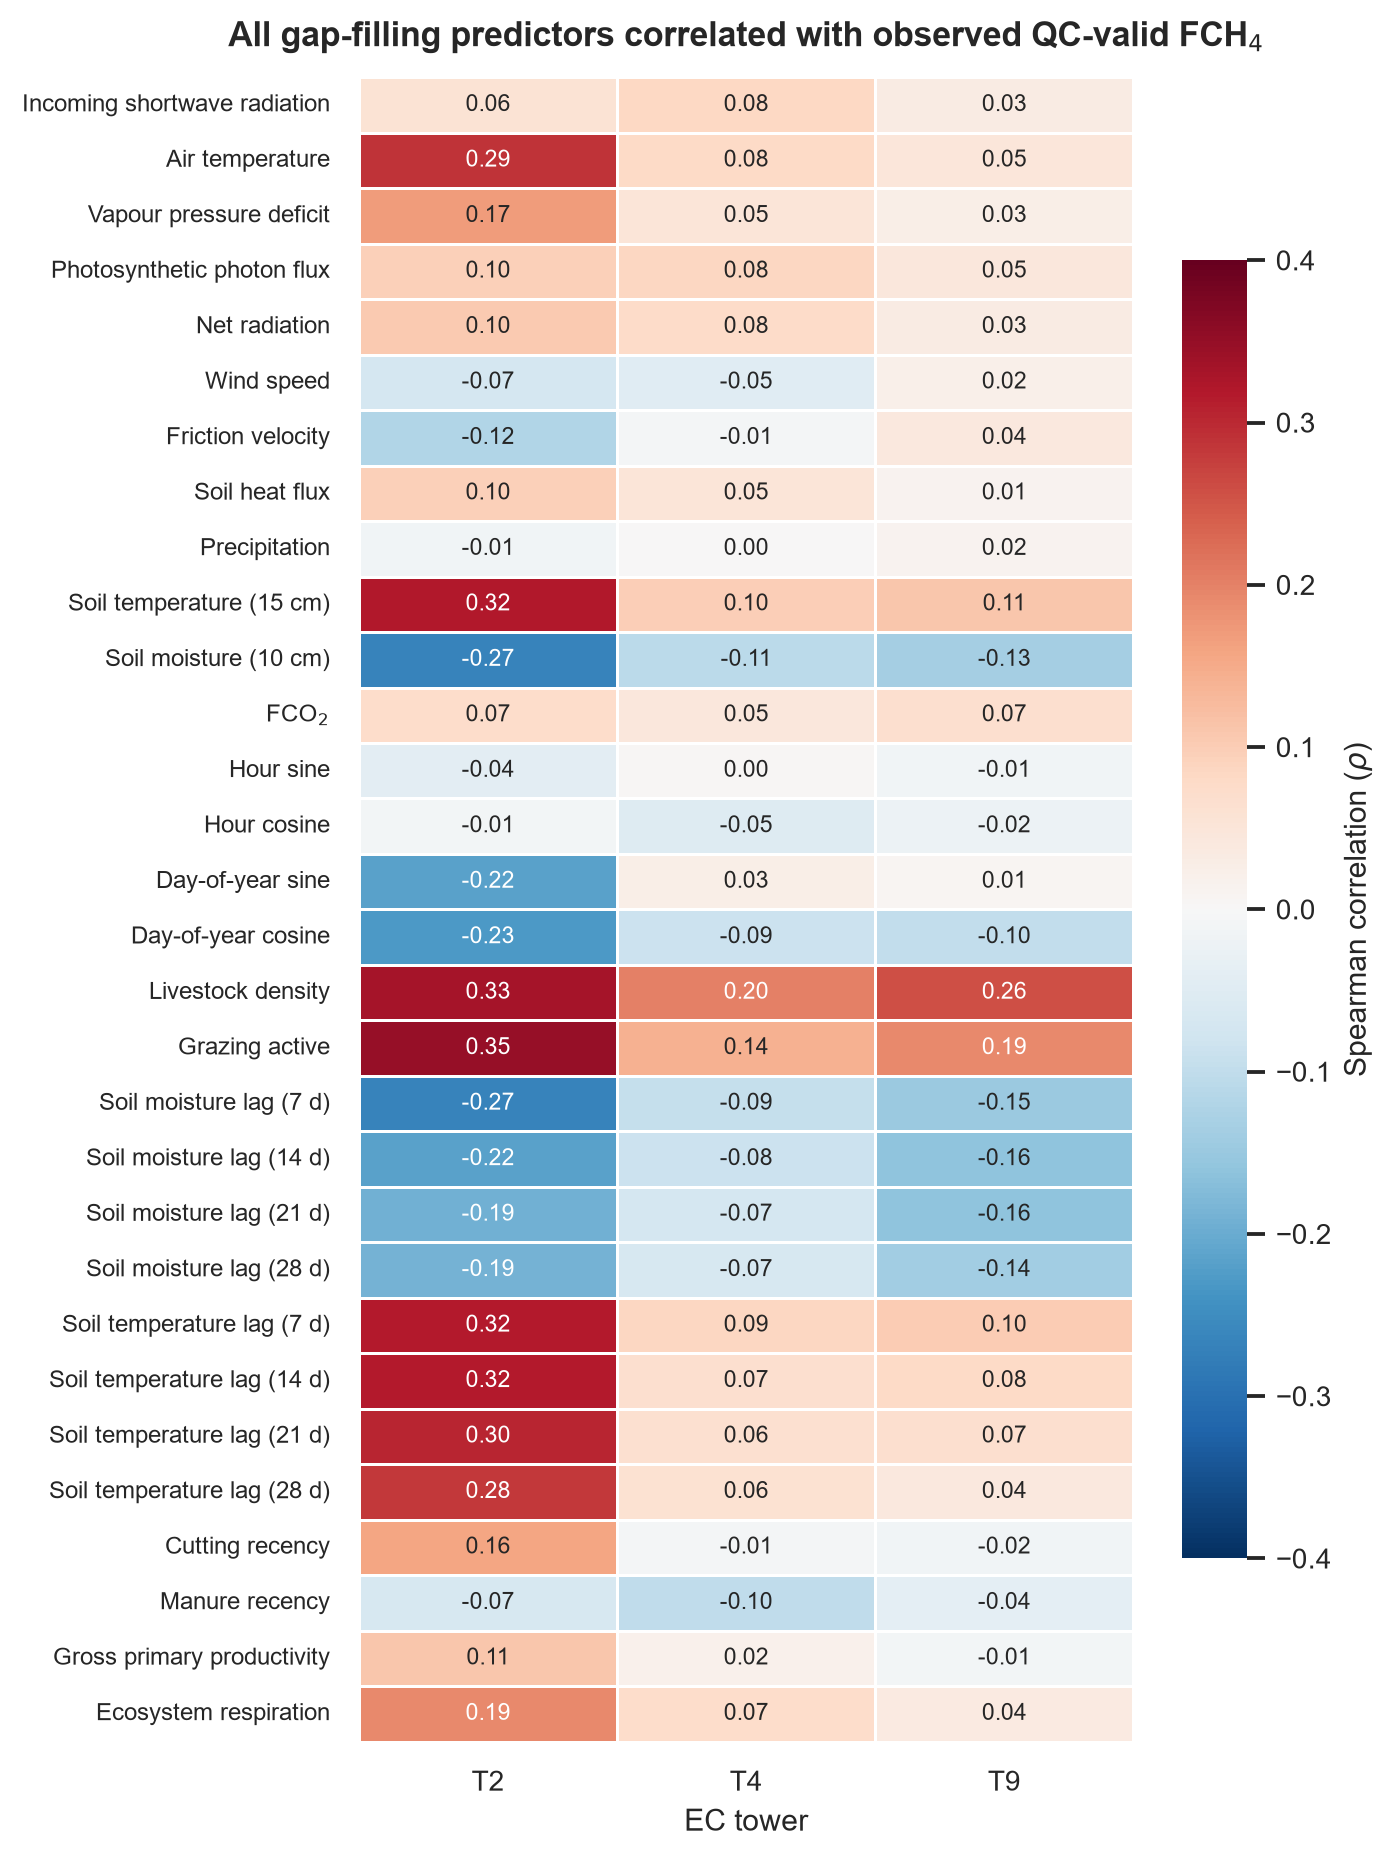
\includegraphics[width=0.82\textwidth]{Figures/ch3_fch4_target_correlations_full.png}
\caption{Complete matrix of tower-specific Spearman correlations between observed QC-valid
FCH\textsubscript{4} and all 30 predictors used by the gap-filling experiments. The reduced matrix
in Figure~\ref{fig:ch3_target_correlations} presents the union of the five largest absolute
correlations within each tower. These coefficients describe pairwise monotonic association and
should not be interpreted as causal effects or model-based feature importance.}
\label{fig:appendix_target_correlations_full}
\end{figure}

\begin{figure}[htbp]
\centering
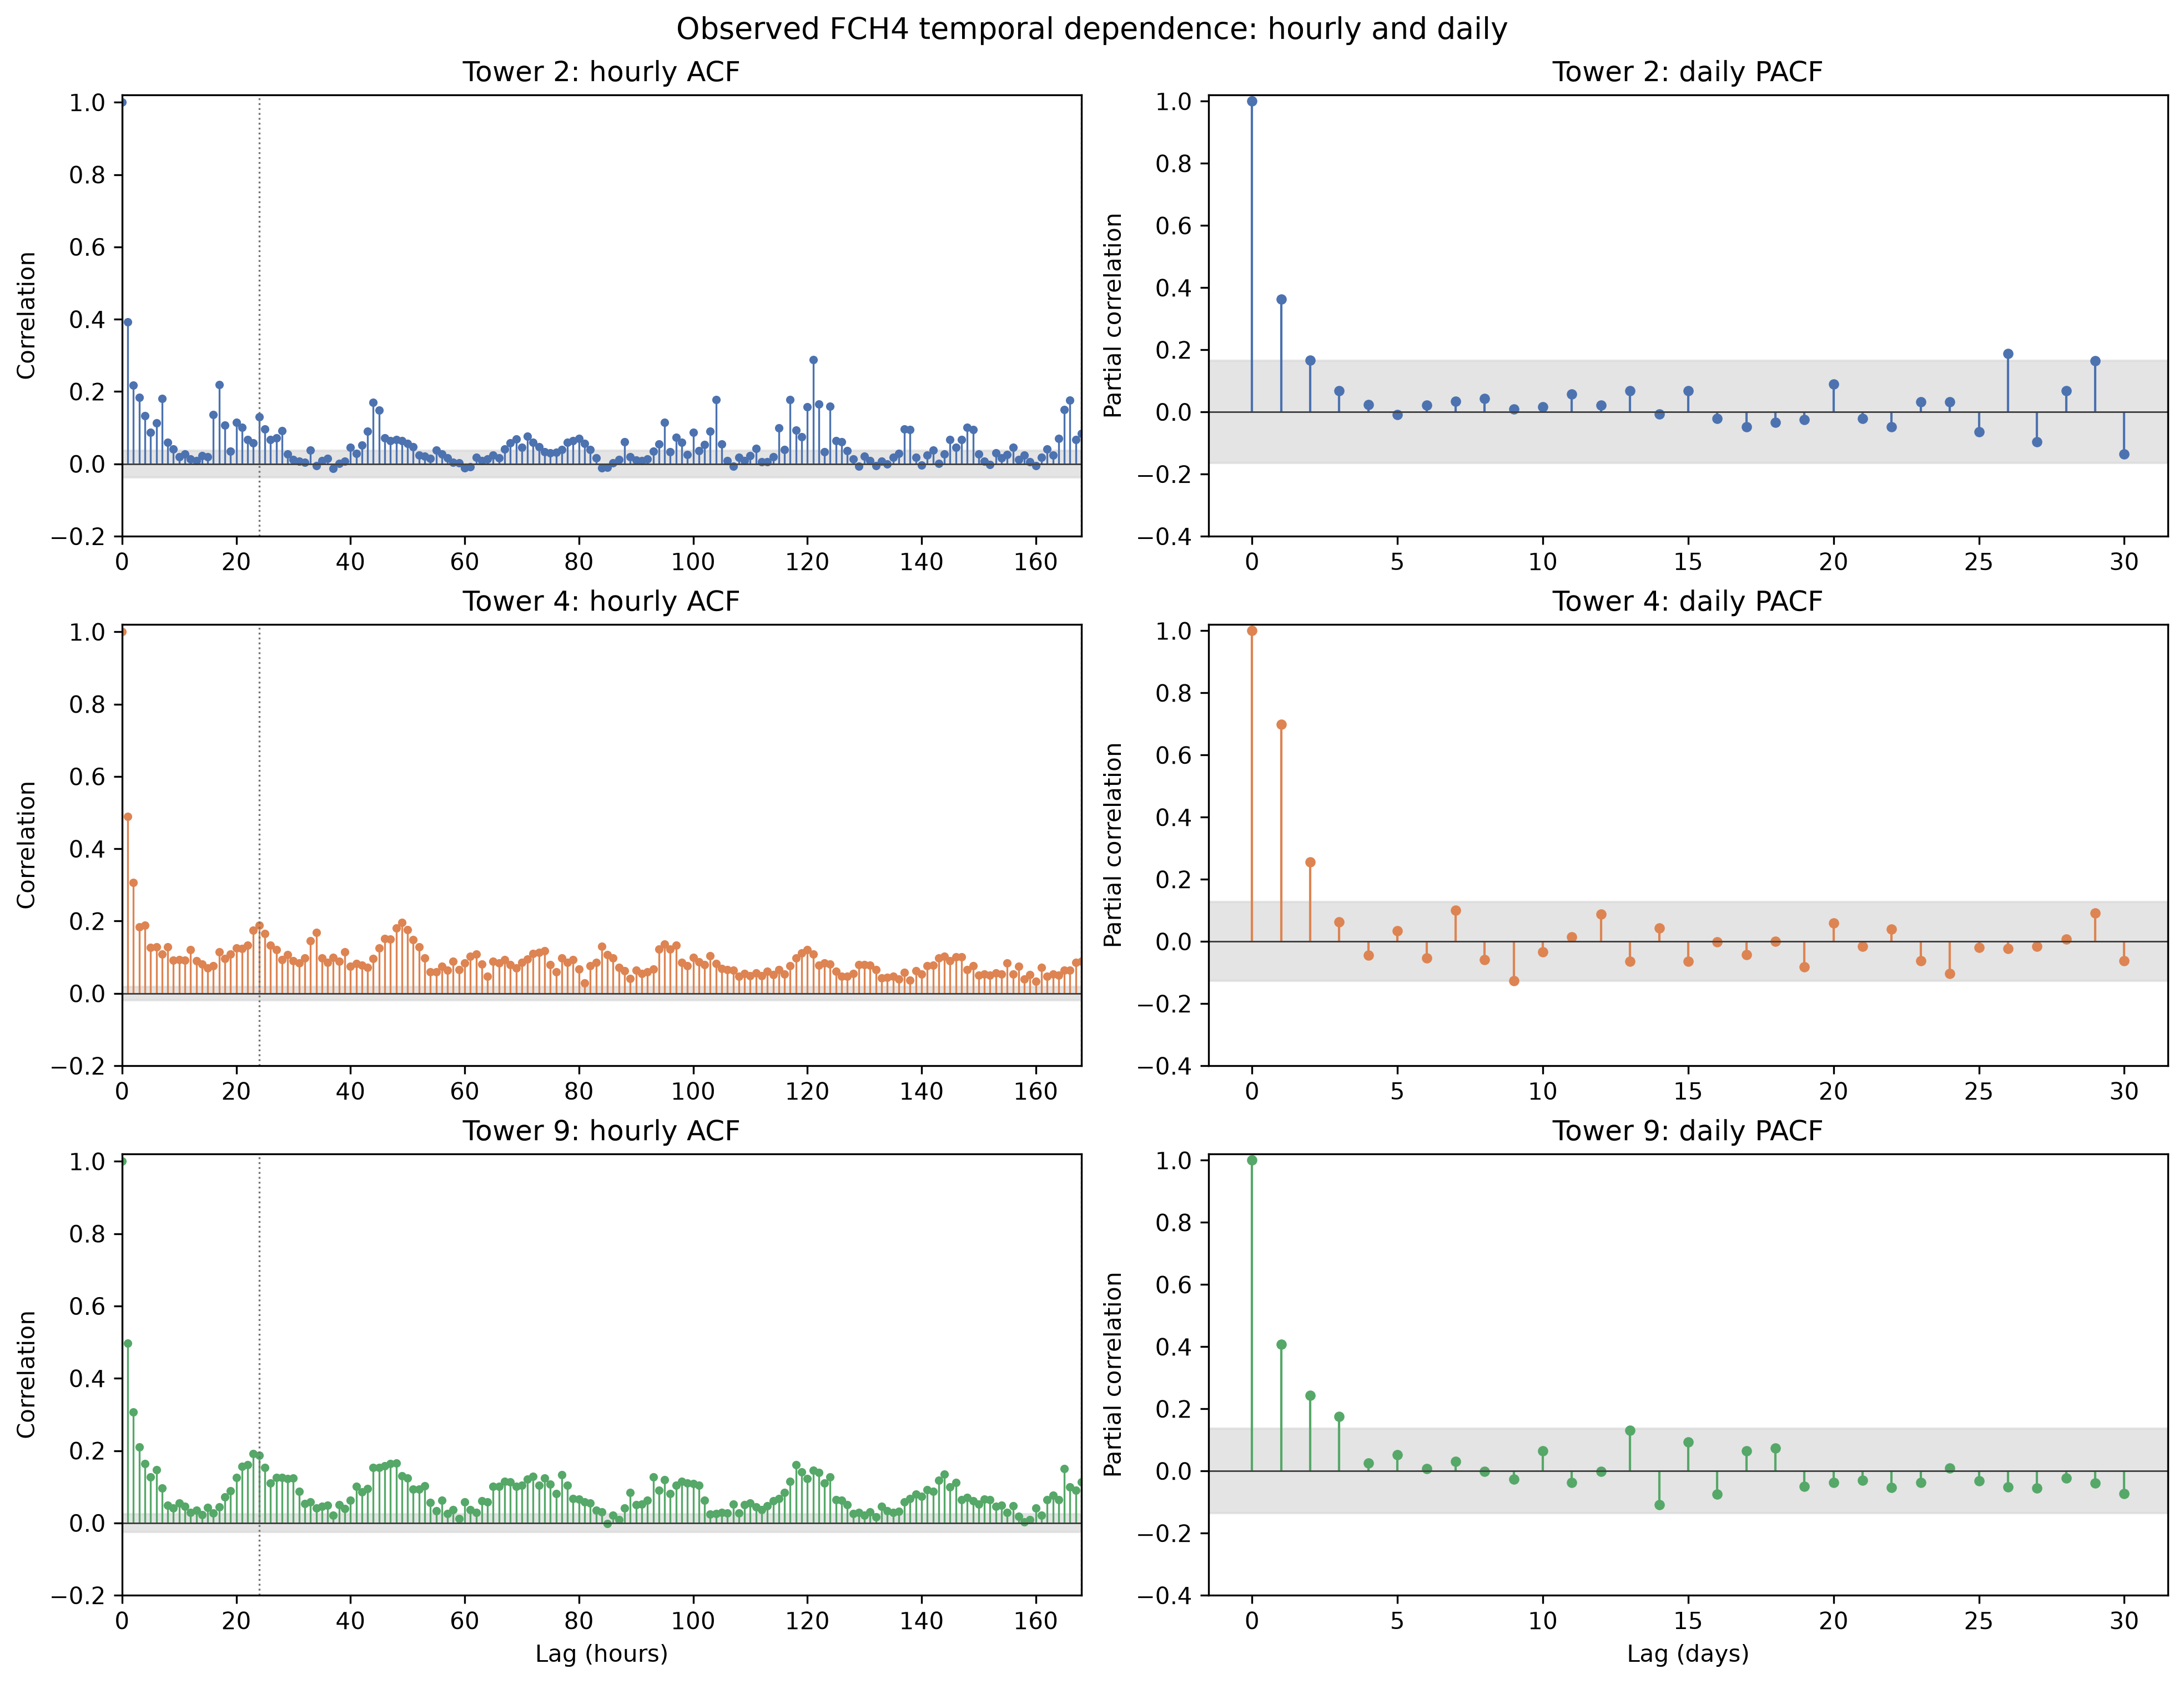
\includegraphics[width=\textwidth]{Figures/ch3_acf_pacf_observed.png}
\caption{
    Temporal dependence of QC-valid observed
  FCH\textsubscript{4}. Left: hourly ACF calculated from available
  observation pairs at each lag, with 24 hours marked by the dotted line.
  Right: daily PACF calculated over the longest sufficiently complete
  segment at each tower; shaded regions show approximate 95\% confidence
  bounds.
}
\label{fig:appendix_ch3_acf_pacf}
\end{figure}

\begin{figure}[htbp]
\centering
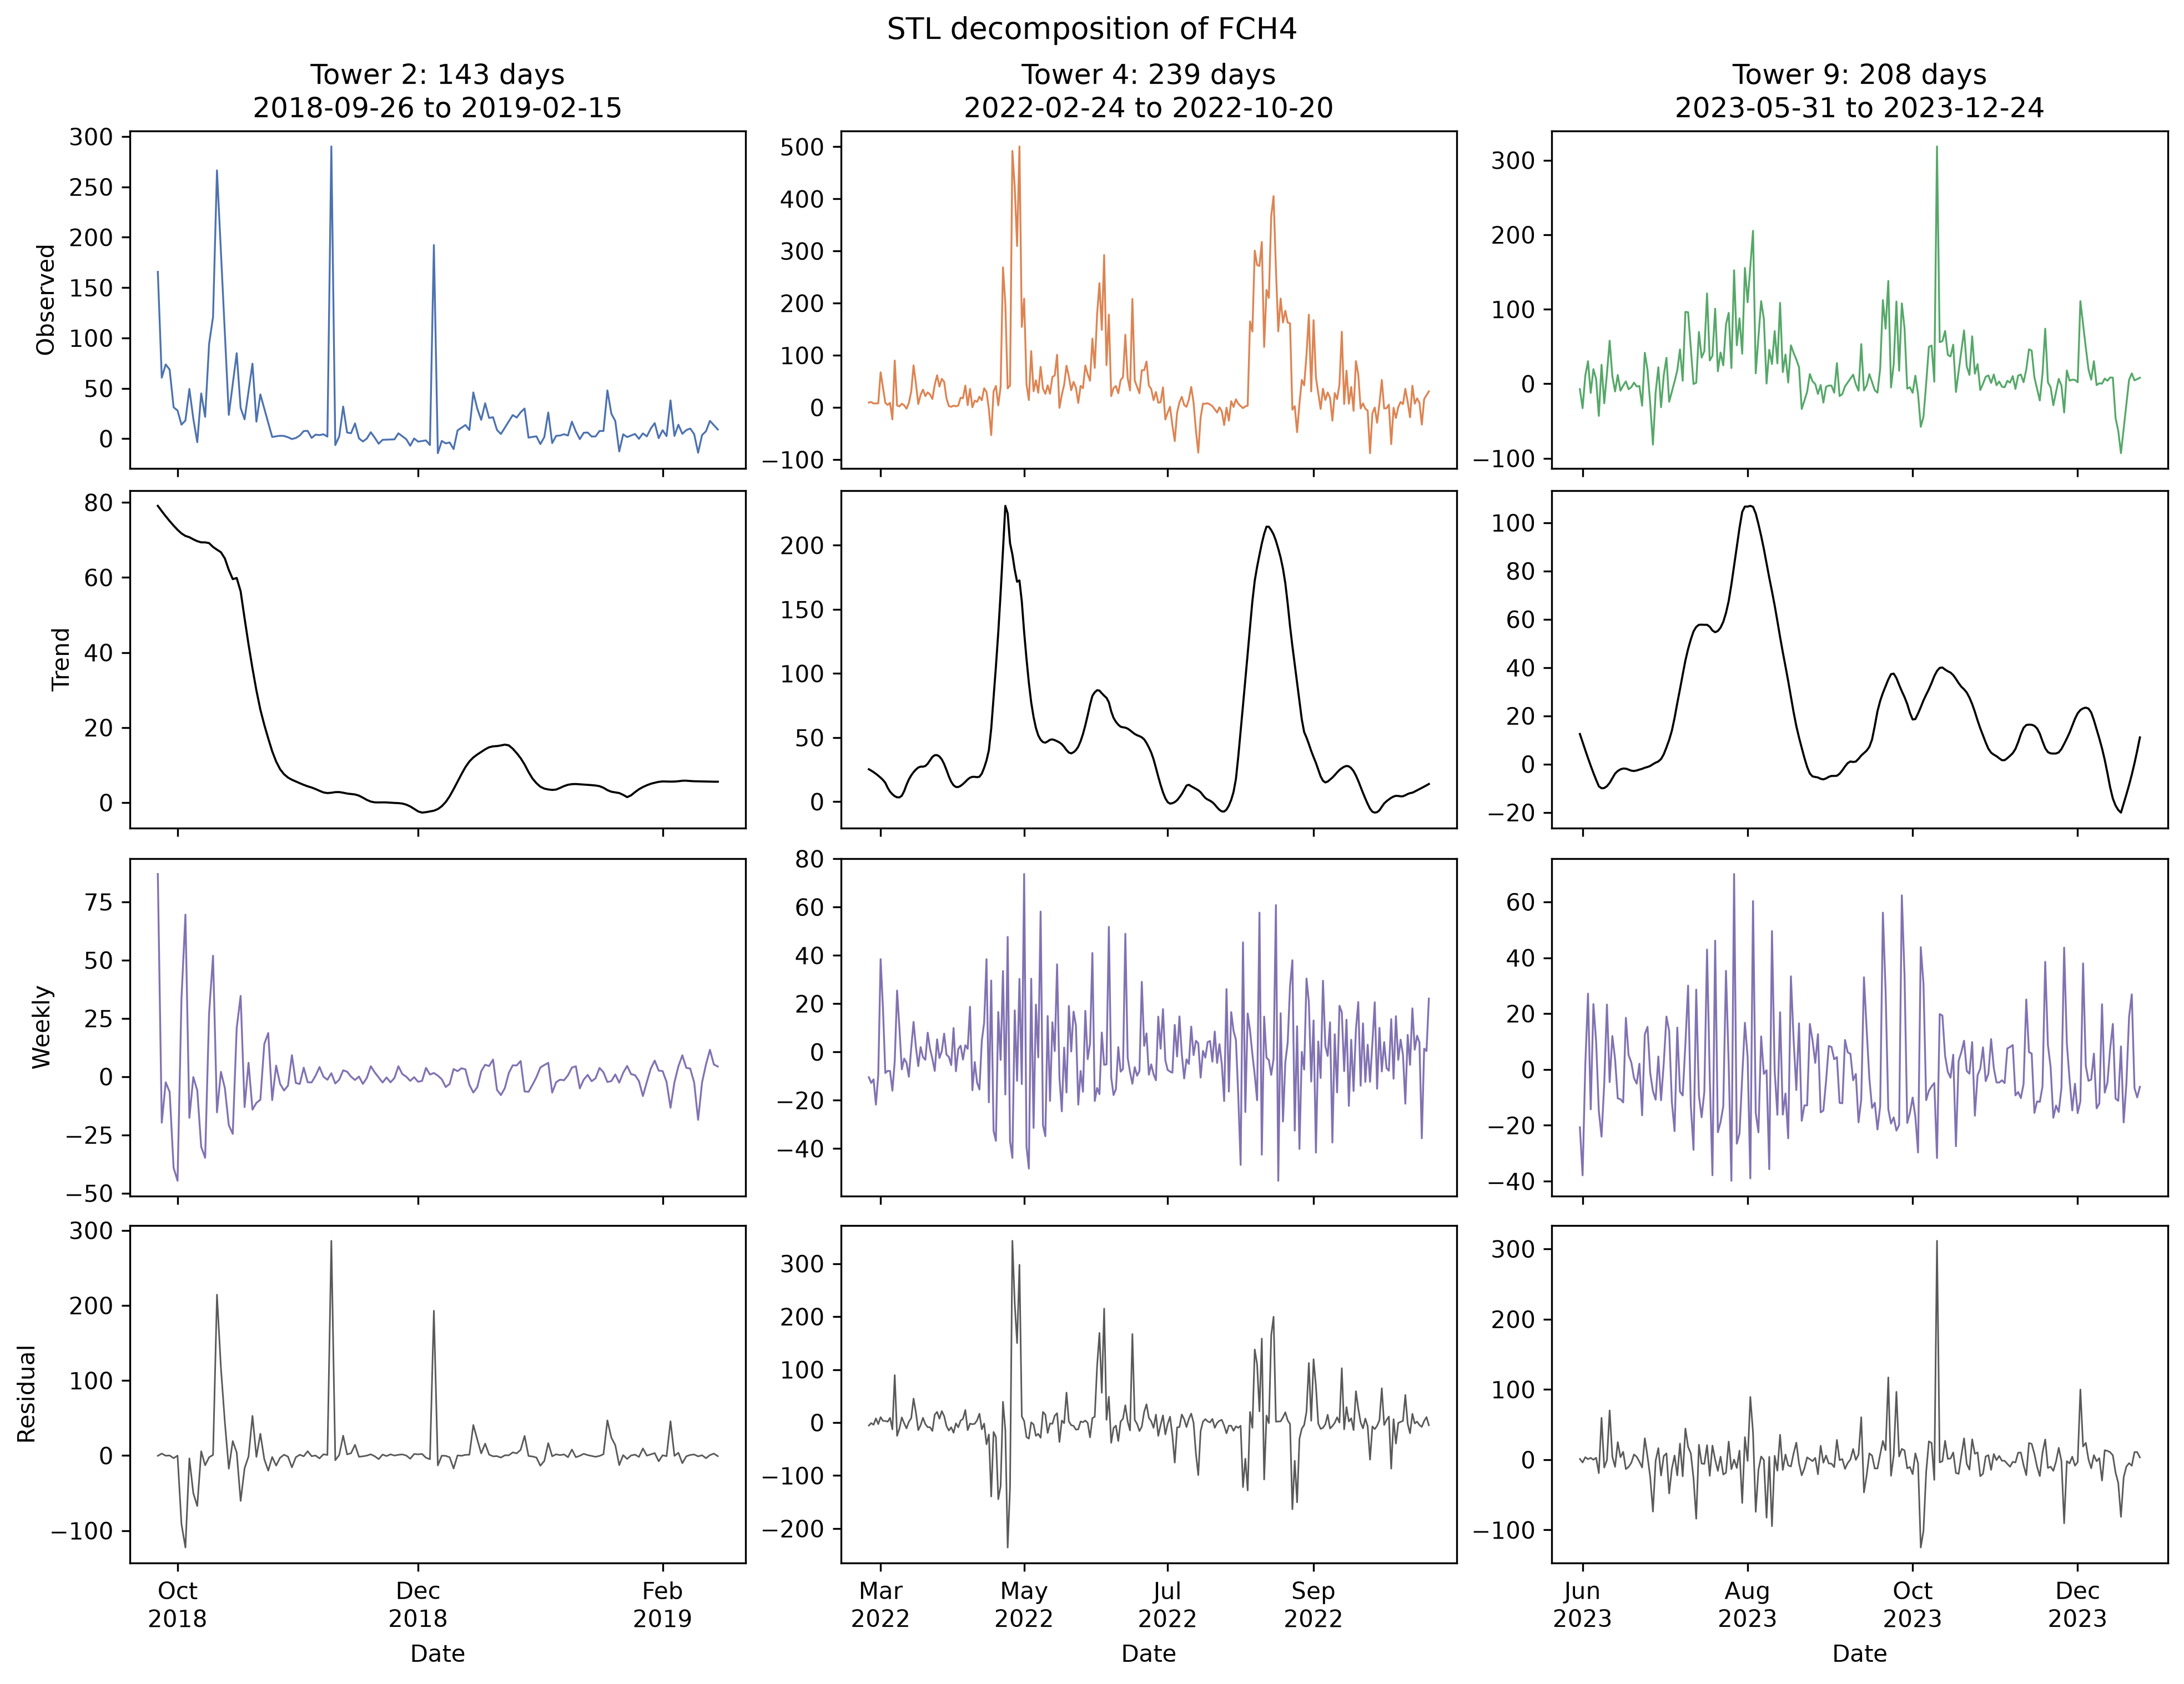
\includegraphics[width=\textwidth]{Figures/ch3_stl_decomposition_observed.png}
\caption{
    Weekly STL decomposition of the longest sufficiently complete
  daily FCH\textsubscript{4} segment at each tower. Rows show the observed
  series, trend, weekly component and residual. 
}
\label{fig:appendix_ch3_stl}
\end{figure}

\FloatBarrier

